%&program=xelatex
%&encoding=UTF-8 Unicode

\documentclass[12pt,oneside,a4paper,titlepage,final]{article}
\usepackage{fontspec}
\usepackage{indentfirst}
\usepackage{setspace}
\usepackage{graphicx}
\usepackage[english]{babel}
\usepackage[pdfborder={0 0 0},pdfpagelabels=true,plainpages=false]{hyperref}
\usepackage[all]{hypcap}

\usepackage{amsmath}
\usepackage{amsthm}

\newtheoremstyle{note}{\parskip}{0pt}{}{\parindent}{\bfseries}{:}{.5em}{}
\theoremstyle{note}
\newtheorem*{warning}{Warning}

% Better quotations
\newcommand*{\uv}[1]{"#1"}

% Metadata
\newcommand{\gettitle}{logdiag}
\newcommand{\getsubtitle}{User Guide}
\newcommand{\getauthor}{Přemysl Janouch}
\newcommand{\getdate}{6. March 2011}

\hypersetup{pdftitle={\gettitle{} --- \getsubtitle},pdfauthor={\getauthor}}

\begin{document}

% Number the first pages with roman numerals
\renewcommand{\thepage}{\roman{page}}

% The title page has no header or footer at all
\thispagestyle{empty}

\begin{center}
	\doublespacing
	\textbf{\LARGE\gettitle}\\{\Large\getsubtitle}
	\par\getauthor
	\par\getdate
	\vfill
	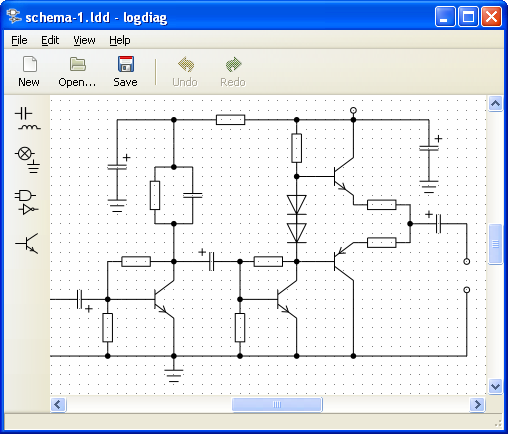
\includegraphics{logdiag-en}
	\newpage
\end{center}

\tableofcontents
\newpage

% Number the real content with arabic numerals and show them in the footer
\renewcommand{\thepage}{\arabic{page}}
\setcounter{page}{1}

\section{Introduction}
This document will guide you through the application and help to familiarize you with it. The description of tasks is preferentially related to the Microsoft Windows operating system, though it's also valid for other operating systems to a certain extent.

\section{Getting the application}
Download the newest version of the application at the following web address: \mbox{\url{http://github.com/pjanouch/logdiag}}.

\begin{figure}[ht]
	\centering
	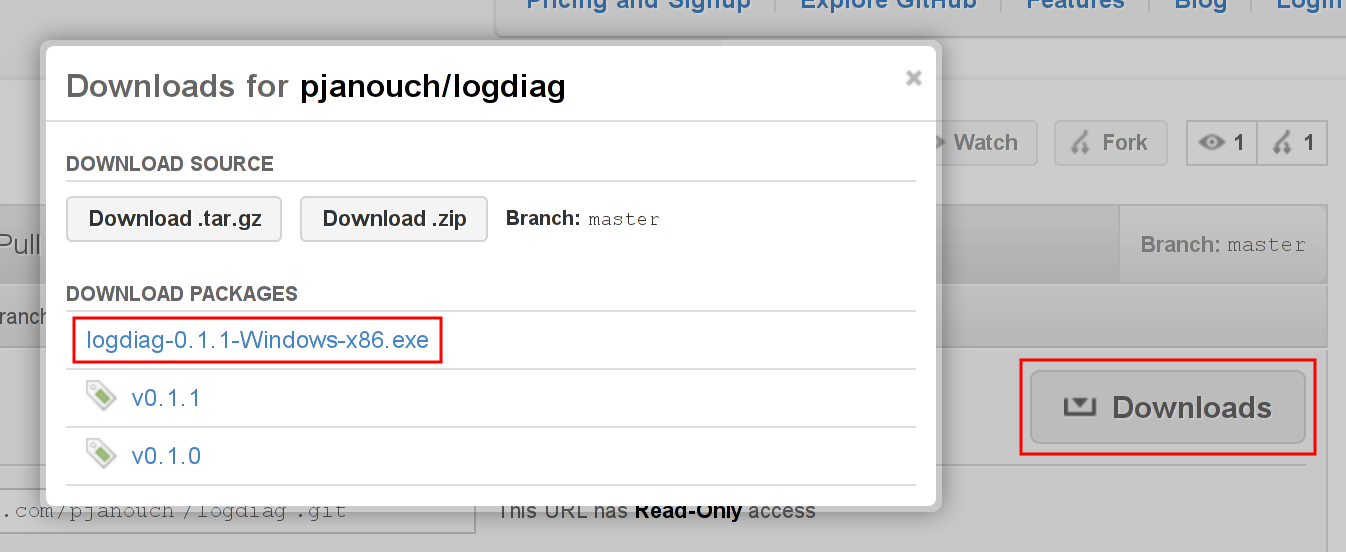
\includegraphics[width=\textwidth,keepaspectratio]{github}
	\caption{The download menu at github}
	\label{github-download}
\end{figure}

While at github, look for a button entitled \uv{Downloads} at the right side of the page and click on it. A menu with packages appears. The installation file for Microsoft Windows is named \uv{logdiag-\emph{version}-Windows-x86.exe}.

\section{Installation}
The installation process is quite straight-forward. After the initial screen the license agreement is required. Next, choose a folder in which to install the application and another one for placement in the Start menu. As long as no unexpected error has occurred, all that's left is confirming a successful installation.

\begin{warning}
	If the application is installed to a folder where a previous installation is already located, problems may arise. Although it is possible to do so, don't try to install multiple copies parallely either, for the same reasons. Remove the current installation first, for example by using the shortcut located in the Start menu.
\end{warning}

\section{Operations with objects}
Each diagram consists of objects, and these are joined with the operations described below. To cancel any current operation, press the Escape key.

\subsection{Selecting objects}
Select single objects by left-clicking on them. They will get highlighted with red color in reaction to this. To select multiple objects, hold the Shift key while clicking.

\begin{figure}[ht]
	\centering
	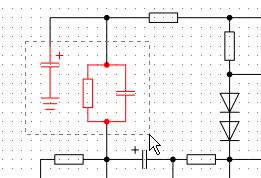
\includegraphics{select-objects}
	\caption{Selecting objects inside an area}
	\label{select-objects}
\end{figure}

Alternatively drag the mouse from free space within the diagram into the area, see figure \ref{select-objects}. Objects contained in this rectangle will be selected. The selection may later be dismissed by just clicking into free space.

\subsection{Moving objects}
Moving of objects is done by dragging them with the mouse onto the desired place. If these objects form a part of the current selection, the whole selection is moved. The selection may also be moved using cursor keys.

\subsection{Removing objects}
Remove objects either by pressing the Delete key or from the application menu.

\subsection{Inserting symbols}
\emph{Symbols} constitute the most important kind of objects. Insert them into the diagram by choosing one from the symbol menu located at the left side of the main application window, see figure \ref{select-symbol}. After clicking on a symbol, click again into the diagram where the symbol is to be placed.

\begin{figure}[ht]
	\centering
	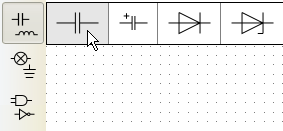
\includegraphics{select-symbol}
	\caption{Choosing a symbol from the menu}
	\label{select-symbol}
\end{figure}

\subsection{Rotating symbols}
Rotate a symbol inserted into the diagram by right-clicking on it.

\subsection{Connecting terminals}
A point intended for creation of connections between symbols or other connections is called a \emph{terminal}. To lead a connection out of it, first hover it with the mouse pointer, so it gets visibly highlighted with a circle. Then press the left mouse button and drag the pointer onto the place where you want the connection to end.

\begin{figure}[ht]
	\centering
	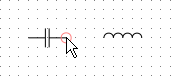
\includegraphics{create-connection-begin} \hspace{15pt} 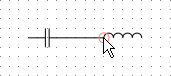
\includegraphics{create-connection-end}
	\caption{Interconnecting terminals of two symbols}
	\label{create-connection}
\end{figure}

\section{Frequent problems}
\subsection{Can't open a saved diagram}
When saving, assure that the filename you've typed in contains the \uv{.ldd} suffix. If not, it won't show up in the dialog for opening diagrams. In case you've already saved a file without an extension, you may fix this situation by adding the suffix to its name.

\subsection{How do I print a diagram?}
The current version of application is not able to print directly. To print out a created diagram, you may use the PrintScreen key to capture a screenshot, then insert it to, for example, Paint, and print it from inside the graphics editor.

\subsection{I miss labels}
Similarly to the previous case, this functionality doesn't exist yet, but it is possible to get around this limitation via a regular graphics editor.

\end{document}


